\section{Propagator Panel}

%------------------------------------------------------------
%--------------  Main Propagator Panel Image ----------------
%------------------------------------------------------------

\begin{figure}[ht]
\begin{center}
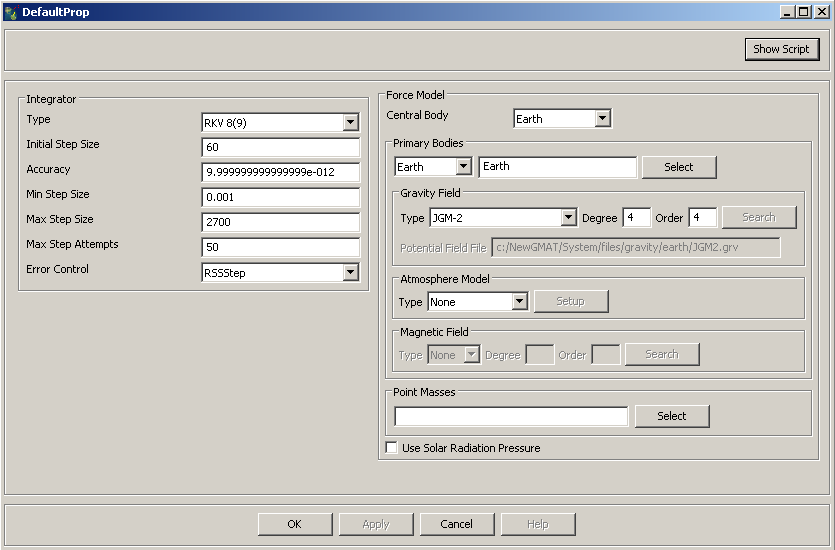
\includegraphics[468,337]{Images/Propagator.png}
\caption{\label{figure:Propagator} The Propagator Panel}
\end{center}
\end{figure}

%------------------------------------------------------------
%--------------  Main Propagator Panel Image ----------------
%------------------------------------------------------------


\textbf{Radio Buttons and Check Boxes}\\

\noindent For the radio buttons and check boxes listed below perform
the tests listed in Table \ref{Table:DataElementTests}:
%
\begin{itemize}
    %
    \item Use Solar Radiation Pressure
    %
\end{itemize}


\noindent\textbf{Combo Boxes}\\

\noindent For the combo boxes listed below perform the tests listed
in Table \ref{Table:DataElementTests}:
%
\begin{itemize}
    %
    \item Integrator/Type
    %
    \item Integrator/Error Control
    %
    \item ForceModel/Central Body
    %
    \item ForceModel/Primary Bodies
    %
    \item ForceModel/Gravity Field/Type
    %
    \item ForceModel/Atmosphere Model/Type
\end{itemize}


\noindent\textbf{Text Fields}\\

\noindent For the text fields listed below perform the tests listed
in Table \ref{Table:DataElementTests}:
%
\begin{itemize}
    %
    \item Integrator/Initial Step Size
    %
    \item Integrator/Accuracy
    %
    \item Integrator/Min Step Size
    %
    \item Integrator/Max Step Size
    %
    \item Integrator/Max Step Attempts
    %
    \item ForceModel/Gravity Field/Degree
    %
    \item ForceModel/Gravity Field/Order
    %
    \item AtmosphereModel/Setup/Solar Flux
    %
    \item AtmosphereModel/Setup/Average Solar Flux
    %
    \item AtmosphereModel/Setup/Geomagnetic Index
    %
    \item AtmosphereModel/FileName
    %
\end{itemize}

\noindent \emph{Select ABM under Integrator/Type to see these Text
Fields}
\begin{itemize}
    %
    \item Integrator/Nominal Integration Error
    %
    \item Integrator/Min Integration Error
    %
\end{itemize}


\noindent\textbf{Buttons}\\

\noindent For the Buttons listed below perform the tests listed in
Table \ref{Table:DataElementTests}:
%
\begin{itemize}
    %
    \item Force Model/Primary Bodies/ Select
    %
    \item Force Model/Atmoshere Model/Setup
    %
    \item Force Model/Point Masses/Select
    %
\end{itemize}



\noindent\textbf{Selection Lists}\\

There are no Selection Lists on the Propagator panel.\\



\noindent\textbf{Tabbed Panels}\\

There are no Tabbed Panels on the Propagator panel\\



\noindent\textbf{Numeric Tests}\\

There are no Numeric Tests for the Propagator panel.\\



\noindent\textbf{Panel Specific Field Coupling Tests}\\

These tests are related to interactions between different data
elements on the panel.\\

\begin{itemize}
    %
    \item Add Sun, Luna, Mercury, and Venus to Primary bodies list.  Now
    click on the Select button under point masses.  Ensure that all
    bodies that appear in the primary bodies list do not appear
    on the selection panel for point masses.
    %
    \item Create a new propagator.  Add Sun, Luna, Mercury, and Venus to point masses list.  Now
    click on the Select button under Primary Bodies.  Ensure that all
    bodies that appear in the point mass list do not appear
    on the selection panel for Primary Bodies.
    %
    \item Create a new propagator.  Add Sun, Luna, Mercury, and Venus to point masses
    list.  Click apply and hit show script and verify that the
    Sun, Luna, Mercury, and Venus appear in the list of
    point masses.
    %
    \item Create a new propagator.  Add Sun, Luna, Mercury, and Venus
    to Primary Bodies list.  Click apply and hit show script and verify that the
    Earth, Sun, Luna, Mercury, and Venus appear in the list of
    primary bodies.
    %
    \item Create a new propagator.  Add Luna, Mars and Venus as Primary Bodies. Now:

    \begin{itemize}
    %
    \item  In the combo for primary bodies select Luna.  Now in the
    Gravity Field/Type combo box, ensure only LP165 and Other appears in
    the options.  Ensure the Atmosphere/Type combo box is
    disabled.
    %
    \item  In the combo for primary bodies select Mars.  Now in the
    Gravity Field/Type combo box, ensure only Mars-50C and Other appears in
    the options. Ensure the Atmosphere/Type combo box is
    disabled.
    %
    \item  In the combo for primary bodies select Venus.  Now in the
    Gravity Field/Type combo box, ensure only MGNP-180U and Other appears in
    the options. Ensure the Atmosphere/Type combo box is
    disabled.
    %
    \item In the combo for primary bodies select Earth. Click the ForceModel/GravityField/Search button.  Select a
    valid gravity model for earth, that is different from the model already in the panel.  Hit
    ok. Verify that the new model is in the text box.  Hit apply and
    show script and verify that the new model is shown in the
    script.
    \end{itemize}

\end{itemize}
